\documentclass[9pt,twocolumn,twoside,pdftex]{optica}

\usepackage{amsthm}
\newtheorem{definition}{Definition}
\newtheorem*{definition*}{Definition}


\setboolean{shortarticle}{false}
\setboolean{minireview}{false}



\title{Dual oxygen and temperature luminescence sensor based on artificial intelligence}

\author[1,2,*]{Francesca Venturini}
\author[2]{Umberto Michelucci}
\author[1]{Michael Baumgartner}

\affil[1]{Institute of Applied Mathematics and Physics, Zurich University of Applied Sciences,
Technikumstrasse 9, 8401 Winterthur, Switzerland}
\affil[2]{TOELT LLC; Birchlenstr. 25, 8600 Dübendorf, Switzerland}

\affil[*]{Corresponding author: francesca.venturini@zhaw.ch}


% To be edited by editor
% \dates{Compiled \today}

%\ociscodes{(300.6280) Spectroscopy, fluorescence and luminescence; (260.3800) Luminescence; (200.4260) Neural networks; (120.0280) Remote sensing and sensors.}

%https://www.osapublishing.org/submit/ocis/#230.0230
% To be edited by editor
% \doi{\url{http://dx.doi.org/10.1364/optica.XX.XXXXXX}}

\begin{abstract}
The optical determination of oxygen partial pressure is of great interest in numerous areas, like medicine, biotechnology, and chemistry. A well-known approach to the optical measure of oxygen is based on the quenching of luminescence by molecular oxygen. Sensors based on this principle typically rely on approximate empirical models to characterize the dependence of the luminescence intensity and decay time on the oxygen concentration through a multi-parametric model (Stern–Volmer equation), whose parameters are, however, all temperature-dependent. Therefore, the temperature needs to be known to determine the oxygen concentration and is measured separately, either optically or with a completely different sensor. In this work, we propose a new artificial intelligence approach, which allows the extraction of both the oxygen concentration and the temperature using one single indicator (luminophore), which is sensitive to both oxygen and temperature, and measuring only the decay time. The results show that the neural network achieves predictions of both parameters, which are comparable to the accuracy of commercial senors and therefore demonstrate the feasibility of this approach. Furthermore, the proposed artificial intelligence approach is not limited to oxygen and temperature sensing but can be applied to the luminescence of multiple luminophores, whenever the underlying mathematical model is not known or too complex to derive the desired quantities from a single measurement.

\end{abstract}

\setboolean{displaycopyright}{true}

\begin{document}

\maketitle

\section{Introduction}

The simultaneous determination of multiple physical quantities can be very advantageous in many sensor applications, for example, when an in-situ or remote acquisition is required. 
If the physical effect on which the measurement method is based presents cross-interference between the desired quantities, their simultaneous determination becomes a necessity.
In particular optical luminescence sensing is particularly attractive for multiple sensing. Using the same measuring principle, several optical elements, like optical fibers and detectors, can be shared in the setup for the detection of more than one parameter, thus allowing a compact and easy sensor design.

The typical approaches to multiple sensing are based on either the use of a single luminescence indicator (luminophore), whose luminescence is sensitive to more than one quantities or the use of several luminophores, one for each quantity, embedded in a substrate and placed in close physical proximity \cite{Stich2010,Borisov2011novel,Kameya2014,Wang2014,Santoro2016,Biring2019}. To be able to determine each quantity separately it may be necessary to determine more than one optical property (e.g., absorption spectrum, emission spectrum, luminescence intensity, decay time). Another possibility is to measure one single optical property using special detection schemes that take advantage of the emission properties of the used used luminophores \cite{Collier2013,Wang2014,Stehning2004,Jorge2008,Biring2019,Moore2006}. 

The problem of dual sensing is particularly relevant in applications that involve oxygen sensing. The determination of oxygen partial pressure is of great interest in numerous fields, like medicine, biotechnology, environmental monitoring, or chemistry since oxygen plays an important role in many processes \cite{Papkovsky2013,Wang2014}. One of the most used optical measuring approaches uses the effect of the dynamical luminescence quenching by oxygen molecules. The measuring principle is based on the measurement of the luminescence of a specific luminophore, whose intensity and decay time are reduced due to collisions with molecular oxygen \cite{Lakowicz2006}.

Sensors based on this principle must rely on approximated empirical models to parametrize the dependence of the measured sensing quantity (e.g., luminescence intensity or decay time) on influencing factors. Among these, temperature is the parameter with the strongest influence since both the luminescence and the quenching phenomena are strongly temperature-dependent. Therefore, today in any optical oxygen sensor the temperature must be continuously monitored, most frequently with a separate sensor, and used to correct the calculated oxygen concentration \cite{Li2015}. This task can be difficult in practical implementation and may be a major source of error in sensors based on luminescence sensing. Another disadvantage of this approach is that the parametrization of the sensor response with temperature is system specific since it depends  on how the sensing element was fabricated and on the sensor itself \cite{Xu1994,Draxler1995,Hartmann1996,Mills1998,Badocco2008,Dini2011}.

In this work, we propose a revolutionary approach based on artificial intelligence. The method enables accurate dual-sensing, using one single luminophore, and measuring a single quantity.
Instead of describing the response of the sensor as a function of the relevant parameters through an analytical model, a neural network  was designed and trained to predict both oxygen concentration and temperature simultaneously.
This new approach is based on multi-task learning (MTL) neural network architectures. These are characterized by common hidden layers, whose output is then the input of multiple branches of task-specific hidden layers. MTL architectures, in facts, can learn correlated tasks \cite{Argyriou2006, Thrun1996, Caruana1997, Zhang2017, Baxter2000, Thung2018} and are flexible enough to be usable in multi-dimensional regressions \cite{Michelucci2019_2}.

The collection of the large amount of data that is needed for the training and test of neural networks cannot be performed by hand. Therefore, a fully automated setup was developed, which both controls the instruments for adjusting the sensing element environment, medium gas concentration and temperature, and collects the sensor response. This allowed to collect enough measurements to train the neural network on real data and to test the sensor performance on other unseen real data.

This work proposes a paradigm shift from the classical description of the response of the sensor through an approximate empirical parametric model to the use of MTL neural networks. 
These will learn the complex inter-parameter dependencies and sensor-specific response characteristics from a large amount of data automatically collected. This new method will enable to build sensors even if they are too complex to be comfortably described by a mathematical model.


\section{Methods}
\label{sec:methods}

\subsection{Luminescence Quenching for Oxygen Determination}
\label{Theory}

Luminescence-based oxygen sensors usually consist of a dye molecule (luminophore) whose luminescence intensity and decay time decrease for increasing O$_2$ concentrations. This reduction is due to collisions of the excited luminophore with molecular oxygen, which thus provides a radiationless deactivation process (collisional quenching). 
In the case of homogeneous media characterized by an intensity decay which is a single exponential, the decrease in intensity and lifetime are both described by the Stern-Volmer (SV) equation \cite{Lakowicz2006}
\begin{equation}
\frac{I_0}{I}=\frac{\tau_0}{\tau}=1+K_{SV} \cdot \left[O_2\right]
\label{SVe}
\end{equation}
where $I_0$ and $I$, respectively, are the luminescence intensities in the absence and presence of oxygen, $\tau_0$ and $\tau$ the decay times in the absence and presence of oxygen, $K_{SV}$ the Stern–Volmer constant and $\left[O_2\right]$ indicates the oxygen concentration.

For practical applications, the luminophore needs to be embedded in a supporting substrate, frequently a polymer. As a result, the SV curve deviates from the linear behavior of equation (\ref{SVe}). This deviation can be due, for example, to heterogeneities of the micro-environment of the luminophore, or to the presence of static quenching \cite{Wang2014}. A scenario that describes this non-linear behavior involves the presence in the substrate of two or more environments, in which the lumineschence is quenched at different rates \cite{Carraway1991,Demas1995}. This multi-site model describes the SV curve as the sum of $n$ contributions as
\begin{equation}
\frac{I_0}{I}=\bigg[ \sum_{i=1}^n
\frac{f_i}{1+K_{SV,i} \cdot \left[O_2\right]}
\bigg]^{-1}
\label{SVe2}
\end{equation}
where $f_i$'s are the fractions of the total emission for each component under unquenched conditions, and $K_{SVi}$'s are the associated effective Stern–Volmer constants. Depending on the luminophore and on the substrate material, the models proposed in the literature may be even more complex \cite{Demas1995,Hartmann1995,Mills1999}.

In most industrial and commercial sensors, the decay time $\tau$ is frequently preferred to intensity measurement because of its higher reliability and robustness \cite{Wei2019}. The determination of the decay time is done most easily in the frequency domain by modulating the intensity of the excitation.  As a result, the emitted luminescence is also modulated but shows a phase shift $\theta$ due to the finite lifetime of the excited state. This method has the advantage of allowing very simple and low-cost implementation and is widely used in commercial applications.

Although the multi-site model was introduced for luminescence intensities, it is frequently also used to describe the oxygen dependence of the decay times \cite{Demas1995,Quaranta2012}. Therefore, in the simplest case of a two-sites scenario, the model can be rewritten in terms of phase shift as \cite{Michelucci2019}
\begin{equation}
\begin{aligned}
\frac{\tan \theta (\omega, T, [O_2])}{\tan \theta_0 (\omega, T)} =& \bigg( \frac{f (\omega , T) }{1+K_{SV1} (\omega , T) \cdot \left[O_2\right]}+ \\
&\frac{1-f (\omega , T) }{1+K_{SV2} (\omega , T) \cdot \left[O_2\right]} \bigg)^{-1} \\
\label{theta_full}
\end{aligned}
\end{equation}
where $\theta_0$ and $\theta$, respectively, are the phase shifts in the absence and presence of oxygen, $f$ and $1-f$ are the fractions of the total emission for each component under unquenched conditions, $K_{SV1}$ and $K_{SV2}$ are the associated Stern–Volmer constants for each component, and $\left[O_2\right]$ indicates the oxygen concentration. It is to be noted that the quantities $\theta_0$, $f$, $K_{SV1}$, and $K_{SV2}$ are all non-linearly temperature dependent \cite{Ogurtsov2006,lo2008,Zaitsev2016} and may result frequency dependent, an artifact of the approximation of the model. Finally, Eq. \ref{theta_full} needs to be inverted to determine $[O_2]$ from the measured quantity $\theta$. The proposed approach defies the need for the mathematical model through the use of neural network approach. However, the structure of Eq. \ref{theta_full} remains relevant to understand the structure of the data and optimize the architecture of the neural network.


\subsection{Experimental Procedure}
\label{Experimental}

The optical setup used in this work for the luminescence measurements is shown schematically in Fig. \ref{fig:setup}. To be able to acquire a large number of data, both the software for the instrument control and for the data acquisition was written using the software LabVIEW by National Instruments. The acquisition procedure is described in detail in Sect. \ref{Data}.

\begin{figure}[t!]
\centering
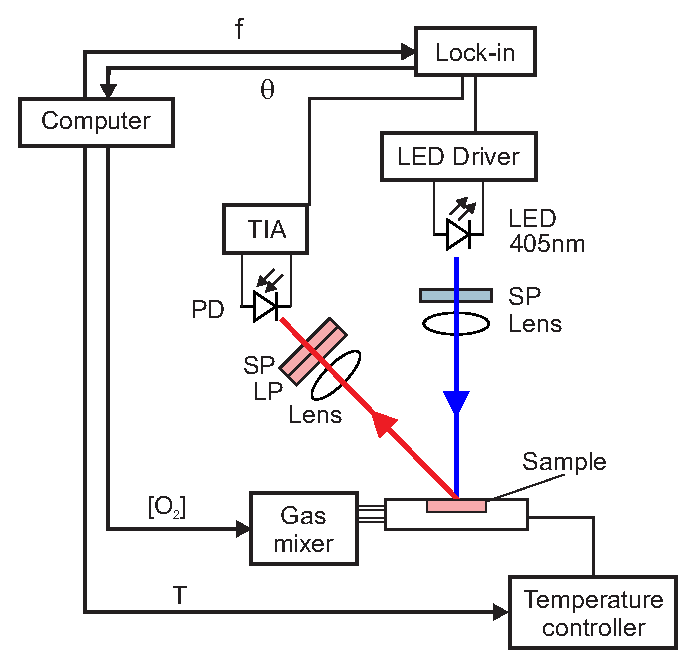
\includegraphics[keepaspectratio, width=8.3cm]{Setup_auto.eps}
\caption{Schematic diagram of the experimental setup. Blue indicates the excitation optical path, red the luminescence one. SP: short-pass filter; LP: long-pass filter PD: photodiode; TIA: trans-impedance amplifier.}
\label{fig:setup}
\end{figure}


\subsubsection{Experimental Setup}

The sample used for the characterization and test is a commercially available Pt-TFPP-based oxygen sensor spot (PSt3, PreSens Precision Sensing).
To control the temperature of the samples, these were placed in good thermal contact with a copper plate, set in a thermally insulated chamber. The temperature of this plate was adjusted using a Peltier element and stabilized with a temperature controller (PTC10, Stanford Research Systems). The thermally insulated chamber was connected to a self-made gas-mixing apparatus which enabled to vary the oxygen concentration between 0 $\%$ and 20 $\%$ vol $O_2$ by mixing nitrogen and dry air from two bottles. In the following, the concentration of oxygen will be given in $\%$ of the oxygen concentration of dry air and indicated with $\%$ air. This means, for example, that 20 $\%$ air was obtained by mixing 20 $\%$ dry air with 80 $\%$ nitrogen and therefore corresponds to 4 $\%$ vol $O_2$. The absolute error on the oxygen concentration adjusted with the gas mixing device is estimated to be below 1 $\%$ air. 
 
The excitation light was provided by a 405 nm LED (VAOL-5EUV0T4, VCC Visual Communications Company LLC), filtered by a short-pass (SP) filter with cut-off at 498 nm (Semrock 498 SP Bright Line HC short pass) and focused on the surface of the samples with a collimation lens. The luminescence was focused by a lens and collected by a photodiode (SFH 213 Osram).
To suppress stray light and light reflected by the sample surface, the emission channel was equipped with a long-pass filter with cut-off at 594 nm (Semrock 594 LP Edge Basic long pass) and a short-pass filter with cut-off at 682 nm (Semrock 682 SP Bright Line HC short pass). The driver for the LED and the trans-impedance amplifier (TIA) are self-made.
For the frequency generation and the phase detection a two-phase lock-in amplifier (SR830, Stanford Research Inc.) was used. 

\subsubsection{Automated Data Acquisition}
\label{Data}

\begin{figure}[b!]
\centering
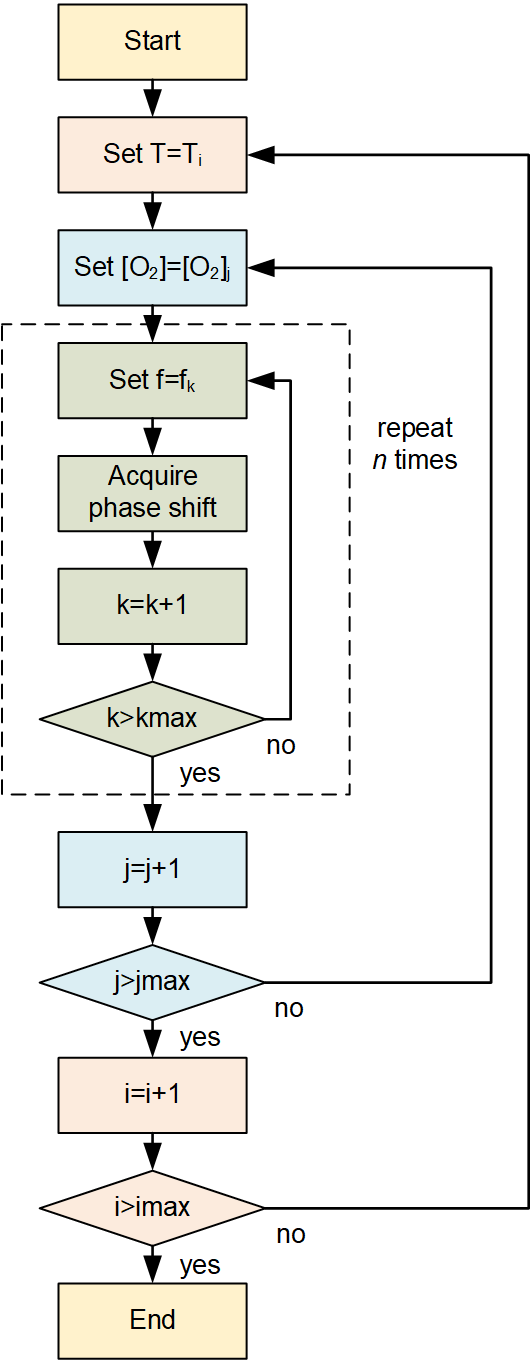
\includegraphics[keepaspectratio, width=5.8 cm]{flow-chart.png}
\caption{Flow-chart of the automated data acquisition program.}
\label{fig:auto-data}
\end{figure}

The large amount of data needed for the training and the test of the neural network was acquired using an automated acquisition program which followed the flow-chart shown in Fig. \ref{fig:auto-data}. First, the program fixed the temperature and concentration. Then, the phase-shift was measured for 50 modulation frequencies between 200 Hz and 15 kHz. This measurement was repeated 20 times. Next, keeping the temperature fixed, the program changed the oxygen concentration and the entire frequency-loop was repeated.
The oxygen concentration was varied between 0 $\%$ air and 100 $\%$ air in 5 $\%$ air steps.
Finally, the temperature was changed, and then the oxygen and frequency loops where repeated. The temperature was varied between 5 $^\circ$C and 45 $^\circ$C in 5 $^\circ$C steps.
The total number of measurements was thus 50 x 20 x 21 x 9 = 189'000, which required a total acquisition time of approximately 65 hours. This number of measurements was chosen as a compromise between maximizing the number of data and avoiding photodegradation, which naturally occurs when the sample is subjected to illumination. At the end of the session, a minimal change in the phase shift was observed.



\subsection{Neural Network Approach}
\label{NN}

The software component of this new sensor type is based on a neural network model (NNM). A NNM is made of three components \cite{Michelucci2017}: a neural network architecture (that includes how neurons are connected, the activation functions and all the hyperparameters), a loss function (here indicated with $L$) and an optimizer algorithm. In this section, those three components are described in detail.

\subsubsection{Neural Network Architecture}

The artificial network used in this work has a multi-task-learning architecture and is depicted schematically in Fig. \ref{fig:NN_MTL_O2_T}. It consists of three {\sl common hidden layers} with 50 neurons, each which generates as output a "shared representation". The name shared representation comes from the fact that the output of common hidden layers is used to predict both $[O_2]$ and $T$. These layers are followed by three branches, one without additional layers to predict $[O_2]$ and $T$ at the same, and two with each two additional {\sl task-specific hidden layers} to predict respectively $[O_2]$ and $T$. The shared representation is the input of two "task-specific hidden layers", that learn how to predict $[O_2]$ and $T$ better. This architecture uses the common hidden layers to find common features beneficial to each of the two tasks. During the training phase, learning to predict $[O_2]$ will influence the common hidden layers and, therefore, the prediction of $T$, and vice-versa. The further task-specific hidden layers learn features specific to each output and therefore improve the prediction accuracy. The number of neurons of each task-specific hidden layer used in this work is five. The activation function is the sigmoid function for all the neurons.  A study of which network architecture works best with this kind of data can be found in \cite{Michelucci2019_2}.

The network was trained with two types of input to test its effectiveness. In the first case, each observation consists of a vector of 50 values defined as
\begin{equation}
\label{input1}
{\pmb \theta}_s = \left(
\frac{\theta(w_1)}{90} , \frac{\theta(w_2)}{90} , ..., \frac{\theta(w_{50})}{90} 
\right)
\end{equation}
where $w_i$ are the 50 values of the modulation frequency of the excitation light (see Sec. \ref{Experimental}).
In the second case, each observation is
\begin{equation}
\label{input2}
{\pmb \theta}_n = \left(
\frac{\theta(w_1)}{\theta_0(w_1)} , \frac{\theta(w_2)}{\theta_0(w_2)} , ..., \frac{\theta(w_{50})}{\theta_0(w_{50})} 
\right)
\end{equation}
where $\theta_0(w_i)$ is the value of the phase shift without oxygen quenching at the modulation frequency $w_i$.

\begin{figure}[t!]
\centering
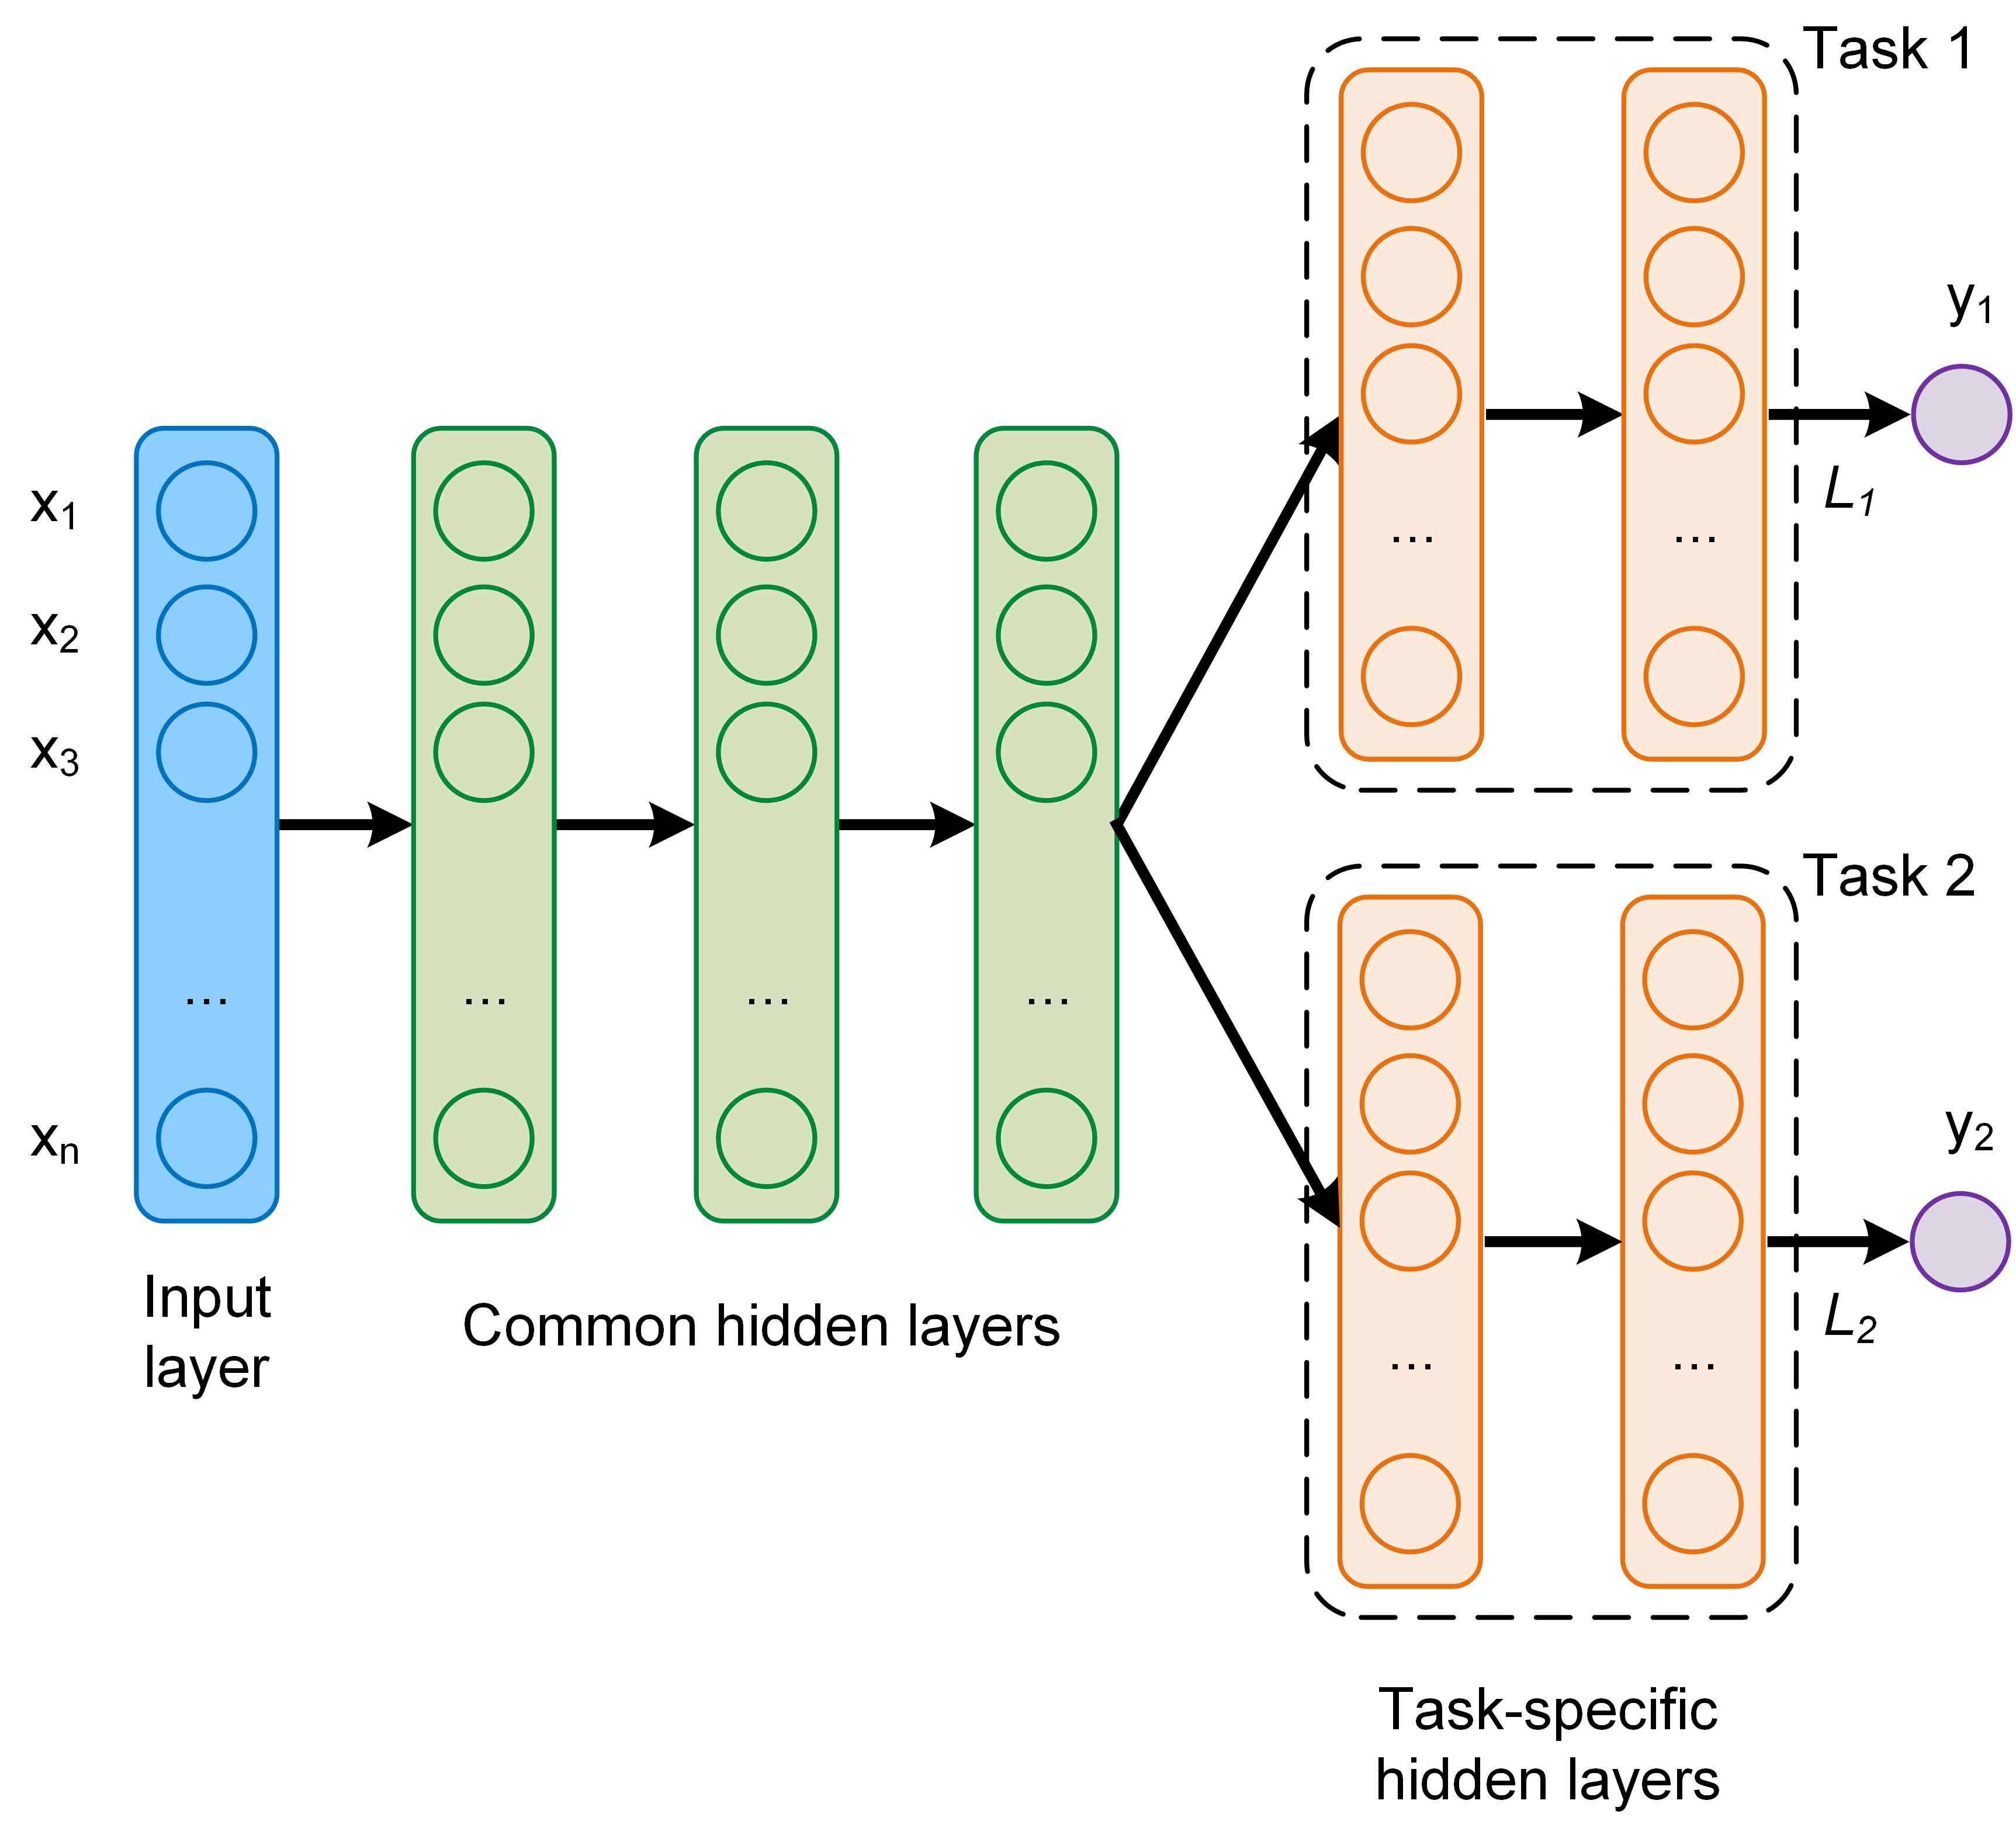
\includegraphics[width=8.7 cm]{NN_MTL.png}
\caption{Architecture of the multi-task learning neural network used in this paper. The common hidden layers generate as output a "shared representation" that is used as input to task specific branches that learn specific features to each quantity and therefore improve the prediction accuracy. $L_i$ are the task-specific loss functions; $[O_2]_{i,pred}$ and $T_{i,pred}$ are the oxygen concentration and temperature predictions of  the corresponding branch $i$. Note that branch 2 and 3 have only one output.} 
\label{fig:NN_MTL_O2_T}
\end{figure}


\subsubsection{Loss Function}

The task-specific loss functions for each branch $i$ is indicated with $L_i$ and is the mean square error (MSE) defined as
\begin{equation}
L_i = \frac{1}{n} \sum_{j=1}^n \sum_{k=1}^{d_i} (y_{k,i}^{[j]}-\hat y_{k,i}^{[j]})^2, \ \ \ i=1,2,3
\label{MSE}
\end{equation}
where $n$ is the number of observations in the input dataset; ${\mathbold y}_i^{[j]} \in \mathbb{R}^{d_i}$ is the measured value of the desired quantity for the $j^{th}$ observation, with $j=1, ..., n$  and $d_i$ is the dimension of the neural network branch output. In this case $d_1=2, d_2=1$ and $d_3=1$. $ \hat {\mathbold y}_i^{[j]} \in \mathbb{R}^{d_i}$ is the output of the network branch $i$, when evaluated on the $j^{th}$ observation. Since there are multiple branches, a global loss function $L$ needs to be defined as a linear combination of the task-specific loss functions with weights $\alpha_i$ 
\begin{equation}
L = \sum_{i=1}^{n_T}\alpha_i L_i .
\label{globalcf}
\end{equation}
The parameters $\alpha_i$ have to be determined during the hyper-parameter tuning phase to optimize the network predictions.
In this paper, being the loss function the MSE (Eq. \ref{MSE}), the global loss function is
\begin{equation}
L = \sum_{i=1}^{3}\alpha_i \frac{1}{n} \sum_{j=1}^n \sum_{k=1}^{d_i} (y_{i,k}^{[j]}-\hat y_{i,k}^{[j]})^2
\end{equation}
The global loss function weights used for this work were $\alpha_1 = 0.3$, $\alpha_2 = 5$ and $\alpha_3 = 1$. These parameters are the result of a hyper-parameter tuning for this architecture \cite{Michelucci2019_2}.
 

\subsubsection{Optimiser Algorithm}
\label{training}

The loss function was minimized using the optimizer Adaptive Moment Estimation (Adam) \cite{Kingma2014, Michelucci2017}. The training was performed with a starting learning rate of $10^{-3}$. Two types of training were investigated to compare the training efficiency and performance of the network. {\sl No-batch training}: with this method all the training data  are used to perform an update of the weights and to evaluate the loss function. The loss function used is given by Eq. (\ref{MSE}) where $n$ is the total number of observations available (3780). {\sl Mini-batch training}: with this method the weight update is performed after the network has seen 32 observations. In this case Eq. (\ref{MSE}) is used with $n=32$. For each weight update, 32 random observations are chosen from the training dataset without repetitions until all the training data were fed to the network.  

No-batch training has the advantage of stability and speed since it performs one weight update using the entire training dataset. Mini-batch training is normally much more effective, allowing to reach smaller values of the loss function in less epochs, but usually takes more time \cite{Michelucci2017}. In our experiments for $20 \cdot 10^3$ epochs No-batch training took roughly five minutes on a modern MacBook Pro, while mini-batch training with $b=32$ took approximately 1 hour, thus resulting ca. 12 times slower. 
The implementation was performed using the TensorFlow\texttrademark $\ $library. 


\subsection{Performance Evaluation}

To evaluate the performance of the sensor, different quantities or metrics were analyzed and are discussed in the next sections.


\subsubsection{Absolute Error on the Prediction}

The metric used to compare predictions from expected values is the absolute error ($AE$) defined as the absolute value of the difference between the predicted and the expected value for a given observation. Note that in the architecture described in the previous sections, only branch 1 and 2 can predict $[O_2]$, while $T$ can be predicted by branch 1 and 3. In what follows, the predicted $[O_2]$ will always be from branch 2, while the predicted $T$ from branch 3. For the oxygen concentration for the 
$j^{th}$ observation $[O_2]^{[j]}$  the $AE$ is 
\begin{equation}
\label{AE}
AE^{{[j]}}_{[O_2]} = |[O_2]^{{[j]}}_{pred}-[O_2]^{[j]}_{meas}|.
\end{equation}
Where $[O_2]^{{[j]}}_{pred}$ and $[O_2]^{{[j]}}_{meas}$ are respectively the $[O_2]$ network prediction and  expected value.
The further quantity used to analyse the performance of the network is the mean absolute error ($MAE$), defined as the average of the absolute value of the difference between the predicted and the expected oxygen concentration or temperature. For example, for the oxygen prediction using the training dataset $S_{train}$, the $MAE_{[O_2]}$ is defined as 
\begin{equation}
\label{MAE}
MAE_{[O_2]}(S_{train}) = \frac{1}{|S_{train}|} \sum_{j \in S_{train}}|[O_2]_{pred}^{[j]}-[O_2]_{real}^{[j]}|
\end{equation}
where $|S_{train}|$ is the size (or cardinality) of the training dataset. 
$AE_{T}$ and $MAE_T$ are similarly defined, using $T$ instead of $[O_2]$.

\subsubsection{Kernel Density Estimation}

A fundamental quantity to study the performance of the network is the prediction distribution of the $AE$s. This metrics carries information on the probability of the network to predict the expected value. Additionally, the kernel density estimate (KDE) of the distributions of the $AE$s for both the oxygen concentration and the temperature was also calculated. KDE is a non-parametric algorithm to estimate the probability density function of a random variable by inferring the population distribution based on a finite data sample \cite{Hastie2009}.  In this work a Gaussian Kernel and a Scott bandwidth adaptive estimation \cite{Sain1996} using the seaborn Python package \cite{Waskom2020} were used.


\subsubsection{Error Limited Accuracy $\eta$}
\label{sektion:ela}

Generally, in a commercial sensor, the accuracy quantifies the performance of the sensor and helps to decide if the chosen device is appropriate for the application of interest. The above-defined metrics ($AE$ and $MAE$) are useful to compare the performance of different NNMs but do not help quantify which error the neural network senor will ultimately have in practice.
For this reason, in this work we introduce a new metric, which we will call Error Limited Accuracy (ELA) and that we indicate with $\eta$.

\begin{definition*}
In a regression problem, given the metric $AE$, and a certain value of it $\hat{AE}$, the ELA  $\eta$ limited by the error $\hat{AE}$ is defined as the number of predictions $\hat y$ of the NNM that lie in the range $|\hat y-y|\leq \hat{AE}$, with $y$ the expected value, divided by the total number of observations. It will be indicated with $\eta(\hat{AE})$. In more mathematical terms, given the set
\begin{equation}
E(\hat{AE}) = \{ \hat y^{[i]} \ {\text with } \ i = 1,..., n\ | \ \ |\hat y^{[i]}-y^{[i]}|\leq \hat{AE} \} 
\end{equation}
$\eta(\hat{AE})$ is defined as
\begin{equation}
\eta(\hat{AE}) = \frac{|E(\hat{AE})|}{n}
\end{equation}
where $|E(\hat{AE})|$ is the cardinality of the set $E(\hat{AE})$ or in other words, the number of its elements.
\end{definition*}

This metric allows interpreting the regression problem as a classification one. $\eta(\hat{AE})$ simply describes how many observations are predicted by the NNM within a given value of the absolute error. In other words it is simply the percentage of predictions that are within a certain error $\hat{AE}$ from the expected values. Finally, if we take $\hat{AE}$ big enough, all the predictions will be classified perfectly, so $\eta(\hat{AE})$ is expected to approach 1 for large $\hat{AE}$ values. The smaller $\hat{AE}$ is, the smaller will be the number of predictions correctly classified.
$\eta(\hat{AE})$.
A special case is the value $AE=\overline{AE}$ for which $\eta(\overline{AE})=1$ because within $\overline{AE}$ the network would predict all the observations correctly. This value ($\overline{AE}$) will give us the biggest error in the sensor predictions.


\section{Results and Discussion}
\label{Results}

\subsection{Luminescence Experimental Results}

\begin{figure}[b!]
\centering

\includegraphics[width=8.2 cm]{phase_O2_T.eps}
\caption{Measured phase shift as a function of the oxygen concentration for selected temperatures at a fixed modulation frequency of 6 kHz. The arrow marks increasing temperatures.}
\label{fig:expdata1}
\end{figure}

As described in Section \ref{Theory}, the phase-shift non-linearly depends on the oxygen concentration according to the Stern-Volmer equation. Additionally, the phase shift depends on the temperature, which influences the luminescence and the collision mechanisms, and on the modulation frequency of the excitation light as described in Eq. \ref{theta_full}. The measured behaviour of the phase shift for variations of these three quantities are shown in the Figs. \ref{fig:expdata1} to \ref{fig:expdata3}.

Fig. \ref{fig:expdata1} shows the measured phase shifts as a function of the oxygen concentration at a constant modulation frequency of 6 kHz and for increasing temperatures. For clarity, the results at selected temperatures are shown. The decrease of the phase shift due to the collisional quenching is clearly visible in all curves. The phase shift is, as expected, also strongly  temperature-dependent. For $[O_2]=0$, in the absence of oxygen, the reduction of the phase shift with increasing $T$ is due to temperature quenching; the influence of temperature becomes stronger at higher oxygen concentration, as a result of the increase of the diffusion rates of oxygen in the sample (substrate?).

For a given oxygen concentration, the phase shift is strongly dependent on the modulation frequency, as it can be seen in Fig. \ref{fig:expdata2}, where the shape of the frequency response is determined by the distribution of decay times of the sample. Again, the reduction of the phase shift with increasing temperatures is not constant but depends on the modulation frequency.

\begin{figure}[t!]
\centering

\includegraphics[width=8.2 cm]{phase_f_T.eps}
\caption{Measured phase shift as a function of the modulation frequency for selected temperatures at a fixed oxygen concentration of $[O_2]=20 \%$. The arrow marks increasing temperatures.}
\label{fig:expdata2}
\end{figure}

For completeness, the effect of the oxygen concentration on the frequency response at a fixed temperature is shown in Fig. \ref{fig:expdata3}. Compared to Fig. \ref{fig:expdata2}, the frequency response of the sample is much stronger affected by the oxygen concentration than by temperature. In other words, the sample has a higher sensitivity to oxygen than to temperature.

\begin{figure}[t!]
\centering

\includegraphics[width=8.2 cm]{phase_f_O2.eps}
\caption{Measured phase shift as a function of the modulation frequency for selected oxygen concentrations at a fixed temperature of $T=25 ^{\circ}$C. The arrow marks increasing oxygen concentrations.}
\label{fig:expdata3}
\end{figure}

The measurements of Figs. \ref{fig:expdata1} to \ref{fig:expdata3} show how similar the curves of the phase shift may look for different values of oxygen, temperature and modulation frequency. This helps to understand why it is not possible from the measurement of the phase shift, or even of the phase shift for varying modulation frequencies, to simultaneously determine both the oxygen concentration and the temperature using Eq. (\ref{theta_full}). The temperature must be known in advance and used to compute the oxygen concentration. This is no longer the case with the artificial intelligence approach, as it will be shown in the next section. 


\subsection{Sensor performance}

First, the effect of the training on the sensor performance was investigated. As described in Sect. \ref{training}, the neural network was trained with no-batches and with mini-batches. For this comparison the network was trained for 20'000 epochs using the input observations ${\pmb \theta}_s$ as defined in Eq. (\ref{input1}). The results for $AE_{[O_2]}$ and $AE_T$ are shown in Fig. \ref{fig:KDE_results_all}(A) and \ref{fig:KDE_results_all}(B), respectively. The blue histogram shows the $AE$ distribution when using no-batch, the gray when using mini-batches of size 32. The KDE profiles help illustrating the features of the histogram. The effect of introducing mini-batches on the performance is extraordinary. The predictions distributions get much narrower, the mean average errors decrease from $MAE_{[O_2]}=2.4$ \% air and $MAE_{T}=3.6^\circ$C to $MAE_{[O_2]}=1.4$ \% air and $MAE_{T}=1.6^\circ$C. Although the performance is significantly improved, from Fig. \ref{fig:KDE_results_all}(A) and \ref{fig:KDE_results_all}(B) it can also be clearly seen that errors as high as approximately 5~\%~air for $[O_2]$ or 12 $^\circ$C for $T$ are possible. While deciding what the right mini-batch size is, training time must be taken into account. Decreasing the mini-batch size has the side effect of increasing the training time. While training the network without batches requires just a few minutes, reducing the mini-batch size to 32 increases the training time to approximately one hour.

\begin{figure*}[htbp]
\centering
\includegraphics[width=17.5 cm]{KDE_results_all.eps}
\caption{Performance of the neural network for the oxygen (panels (A), (C) and (E)) and for the temperature (panels (B), (D) and (F)) predictions. In all panels the normalized prediction distribution histogram (columns), the kernel density estimate (KDE) of the distribution of the $AE$s (solid line), and $MAE$ (dashed vertical line) are shown. Panels (A) and (B): Comparison between training using no batches (NB) and using mini-batches (MB) with a batch size of 32 for 20'000 epochs; the input of the network is ${\pmb \theta}_s$. Panels (C) and (D): Comparison between training using mini-batches (MB) with a batch size of 32 for 100'000 and 20'000 epochs; the input of the network is ${\pmb \theta}_s$. Panels (E) and (F): 
training using mini-batches (MB) with a batch size of 32 for 20'000 epochs; the input of the network is ${\pmb \theta}_n$.}
\label{fig:KDE_results_all}
\end{figure*}

Fig. \ref{fig:KDE_results_all}(C) and \ref{fig:KDE_results_all}(D) show the comparison between prediction distributions with 20'000 and 100'000 epochs (always using a mini-batch of size 32) using the input observations ${\pmb \theta}_s$ as defined in Eq. (\ref{input1}). The effect of a longer training is a dramatic improvement in the performance. When the network was trained for 100'000 epochs the mean average errors are reduced to only $MAE_{[O_2]}=0.22$ \% air and $MAE_{T}=0.27^\circ$C. Additionally, all the predictions for $[O_2]$ lie below 0.94 \% air, and for $T$ lie below 2.1 $^\circ$C.

The results of Fig. \ref{fig:KDE_results_all}(C) and \ref{fig:KDE_results_all}(D) demonstrate two new findings: 1) with the proposed approach, it is possible to predict both $[O_2]$ and $T$ at the same time from a the phase shift using a single luminophore; 2) that the prediction have expected errors which are comparable or below the typical accuracy of commercial sensors. The possibility of dual sensing paves the road to the development of a completely new generation of sensors.
The price to pay is that to train a network for so many epochs requires, on a modern laptop, approximately 5 hours.

To investigate if the training can be performed more efficiently, the normalized phase shift ${\pmb \theta}_n$ defined in Eq. (\ref{input2}) where used as input to the network. The performance of the network in this case, with a mini-batch size of 32 and a training of 20'000 epochs is shown in Fig. \ref{fig:KDE_results_all}(E) and \ref{fig:KDE_results_all}(F). The performance is further improved; even if the training is only 20'000 the mean average errors are better than what obtained with ${\pmb \theta}_s$ as input and a training of 100'000 epochs: $MAE_{[O_2]}=0.13$ \% air and $MAE_{T}=0.24^\circ$C. The distributions are also narrower, particularly for the temperature. Additionally all the $AE_{[O_2]}$ lie below 0.87 \% air, and  $AE_{T}$ below 1.7 $^\circ$C. This type of training is clearly more efficient. The reason may lie in the additional information which is fed to the network when using the input ${\pmb \theta}_n$ and in the simplified functional behavior of ${\pmb \theta}_n$ compared to ${\pmb \theta}_s$ as it may be expected by Eq. \ref{theta_full}. xxxEXPLAIN BETTERxxxx

The performance of the different neural networks is summarized in Table \ref{TableMAE_summary}. 
\begin{table}[hbt]
\centering
\caption {\bf Summary of the performance for neural network models}

\begin{tabular}{ cccc}
\smallskip 
 Input & Epochs / Batch size & $MAE_{[O_2]}$ & $MAE_{[T]}$  \\ 
 \hline
${\pmb \theta}_s$ & 20'000 / \textrm{no batch} & 2.4 \% air & 3.6 $^\circ C$\\ 
${\pmb \theta}_s$ & 20'000 / 32 & 1.4\% air & 1.6 $^\circ C$\\ 
${\pmb \theta}_s$& 100'000 / 32 & 0.22 \% air & 0.27 $^\circ C$\\ 
${\pmb \theta}_n$ & 20'000 / 32 & 0.13 \% air & 0.24 $^\circ C$\\ 
\end{tabular}
\label{TableMAE_summary}
\end{table}

\subsection{Error Limited Accuracy Plots}

\begin{figure*}[t!]
\centering

\includegraphics[width=15.5 cm]{ELA_comparison_O2_T.eps}
\caption{Comparison of the ELA $\eta$: Panel (A) oxygen prediction, panel (B) temperature prediction. The black line are the results for the network that were trained with ${\pmb \theta}_n$ as input for 20'000 epochs with mini-batchs of size 32, while the red one with ${\pmb \theta}_s$ as input for 100'000 epochs with mini-batchs of size 32. The dashed lines indicates the values of the $\overline{AE}$ for which the predictions would give $\eta=1$.}
\label{fig:ELA_result_comparison}
\end{figure*}

The metrics discussed in the previous sections are useful to compare the network performance and to measure how good the predictions are. However they do not offer an understanding on what a sensor build with such a model could achieve. For practical applications, the relevant question is what is the maximum error which the sensor will have in predicting the oxygen concentration and temperature. To answer this question we introduce a completely new metric: the ELA ($\eta$), as defined in Sect. \ref{sektion:ela}. As explained previously, $\eta$ is defined depending on the chosen metric $m$. In this section the metric chosen is $m=AE_{[O_2]}$ for the oxygen concentration and $m=AE_{T}$ for the temperature. This new metrics will allow the determination of the maximum error of the sensor. 

Fig. \ref{fig:ELA_result_comparison} displays the ELA $\eta(\widehat {AE})$ for oxygen concentration (A) and for the temperature (B). In each panel the results obtained using the input ${\pmb \theta}_n$ and a training for 20'000 epochs are shown in black, and the results obtained using the input ${\pmb \theta}_s$ and a training for 100'000 epochs in red. In both cases the training was performed with mini-batches of size 32.
The dashed lines indicate the values of the $\overline{AE}_{[O_2]}$ and $\overline{AE}_{T}$ for which the error limited accuracy $\eta$ equals 1. In other words, all the predictions will have an error equal or smaller than $\overline{AE}$.
The values of $\overline{AE}_{[O_2]}$ and $\overline{AE}_{T}$ are summarized in Table \ref{table:ela}.

\begin{table}[t!]
\centering
\caption {\bf Summary of the values of $\overline{AE}$ for the cases shown in Fig. \ref{fig:ELA_result_comparison}(A) and \ref{fig:ELA_result_comparison}(B).}

\begin{tabular}{ cccc}
\smallskip 
 Input & Epochs / Batch size & $\overline{AE}_{[O_2]}$ & $\overline{AE}_{T}$  \\ 
 \hline
${\pmb \theta}_s$ & 100'000 / 32 & 0.95 \% air & 2.1 $^\circ C$\\ 
${\pmb \theta}_n $ & 20'000 / 32 & 0.87\% air & 1.7 $^\circ C$\\ 

\end{tabular}
\label{table:ela}
\end{table}

Fig. \ref{fig:ELA_result_comparison}(A) shows that, for the network trained with ${\pmb \theta}_s$ as input, the model would predict perfectly all the oxygen concentrations within 0.95 \% air error. For the network trained with ${\pmb \theta}_n$ this value is futher reduced to 0.87 \% air. This can be interpreted as the accuracy a sensor based on this NNM  would have.
Fig. \ref{fig:ELA_result_comparison}(B) shows the results of the same analysis for the temperature measurement. The interpretation is similar to the one given above for the oxygen concentration predictions. For the network trained with ${\pmb \theta}_s$ as input, the model would predict perfectly all the temperature values within $\overline{AE}_{T}=2.1^\circ$C error. For the network trained with ${\pmb \theta}_n$ this value would be  $\overline{AE}_{T}=1.7^\circ$C. 
%It is interesting to note, that the difference of the two types of input used is not significant in the case of temperature.



\section{Conclusions}

The results in the prediction of the oxygen concentration and temperature show unprecedented accuracy for both parameters, demonstrating that this approach will make a new generation of sensors possible for dual or even multiple sensing. The unprecedented accuracy in predicting both $AE_{[O_2]}$ and $T$ at the same time, from the same set of data, will allow sensors to become easier to build, since no separate temperature measurements are necessary anymore. To be able to estimate what kind of sensor one could build with a given NNM, in this paper a new metric, the ELA ($\eta(\hat m)$), was proposed to be able to estimate how many predictions like within a certain value of the chosen metric from the expected values.


%\section*{Funding Information}
%National Science Foundation (NSF) (1263236, 0968895, 1102301); The 863 Program (2013AA014402).

%\section*{Acknowledgments}


\section*{Disclosures}

\medskip

\noindent\textbf{Disclosures.} The authors declare no conflicts of interest.


% Bibliography
\bibliography{bibliography}

% Full bibliography will be added automatically on a new page for Optics Letters submissions. This command is ignored for journal article submissions.
% Note that this extra page will not count against page length.
\bibliographyfullrefs{bibliography}

%\printbibliography

%Manual citation list
%\begin{thebibliography}{1}
%\bibitem{Michelucci2017}
%Michelucci, U.
%{\sl Applied Deep Learning - A Case-Based Approach to Understanding Deep Neural Networks}; Apress Media, LLC: New York, NY, USA, 2018; pp. 374--375.

%\bibitem{Kingma2014}
%Kingma, D.P.; Ba, J.
%Adam: A method for stochastic optimization. In Proceedings of 3rd International Conference on Learning Representations, ICLR 2015, San Diego, CA, USA, May 7-9, 2015, pp. 1--15.

%\bibitem{Michelucci2019}
%Michelucci, U.; Baumgartner, M.; Venturini, F.
%Optical oxygen sensing with artificial intelligence.
%{\sl Sensors} {\bf 2019}, {\sl 19}, 777.

˜
%\bibitem{Zhang:14}
%Y.~Zhang, S.~Qiao, L.~Sun, Q.~W. Shi, W.~Huang, %L.~Li, and Z.~Yang,
 % \enquote{Photoinduced active terahertz metamaterials with nanostructured
  %vanadium dioxide film deposited by sol-gel method,} Opt. Express \textbf{22},
  %11070--11078 (2014).
%\end{thebibliography}

\end{document} 